% =====================================================================
%  Module Data Lakehouse -- Support 0 : Installation de l'environnement
%  Compilation : pdflatex (2 passes)
% =====================================================================
\documentclass[11pt,a4paper]{article}

\usepackage[utf8]{inputenc}
\usepackage[T1]{fontenc}
\usepackage[french]{babel}
\usepackage{lmodern}
\usepackage[babel=true]{microtype}

\usepackage[a4paper,margin=2.3cm,headheight=14pt]{geometry}
\usepackage{fancyhdr}
\usepackage{titlesec}
\usepackage{needspace}
\usepackage{enumitem}
\usepackage{amssymb}

\usepackage[table]{xcolor}
\usepackage{booktabs}
\usepackage{tabularx}
\usepackage{array}
\usepackage{tikz}
\usetikzlibrary{positioning,arrows.meta,shapes.geometric,babel}
\usepackage{listings}

\usepackage[htt]{hyphenat}
\usepackage[hidelinks]{hyperref}
\usepackage{xurl}
\usepackage{graphicx}
\usepackage{caption}
\usepackage{xltabular}
\usepackage{float}
\captionsetup{font=small,labelfont=bf,labelsep=period}
\graphicspath{{images/}}
% Logos des logiciels (docs/images/logos/, voir LISEZMOI.md) ; sans le fichier, rien ne s'affiche
\newcommand{\logo}[2][1.15em]{\IfFileExists{images/logos/#2.png}{\raisebox{-0.22em}{\includegraphics[height=#1]{logos/#2.png}}\hspace{0.3em}}%
  {\IfFileExists{logos/#2.png}{\raisebox{-0.22em}{\includegraphics[height=#1]{logos/#2.png}}\hspace{0.3em}}{}}}

\setlength{\parskip}{0.5em}
\setlength{\parindent}{0pt}
\setlength{\emergencystretch}{3em}

% ---------- Couleurs ----------
\definecolor{lhblue}{HTML}{1F4E79}
\definecolor{lhteal}{HTML}{0F766E}
\definecolor{lhred}{HTML}{B91C1C}
\definecolor{lhviolet}{HTML}{6D28D9}
\definecolor{lhgray}{HTML}{F3F4F6}
\definecolor{lhbronze}{HTML}{A16207}
\definecolor{lhsilver}{HTML}{64748B}
\definecolor{lhgold}{HTML}{CA8A04}
\definecolor{lhfonce}{HTML}{17394D}
\definecolor{lhvert}{HTML}{5FB89D}
% Pictogrammes de la figure d'architecture (dessins génériques)
\tikzset{
  pics/fichier/.style={code={%
    \fill[white,draw=lhfonce,line width=0.7pt] (-0.32,-0.42) -- (0.18,-0.42) -- (0.32,-0.28) -- (0.32,0.42) -- (-0.32,0.42) -- cycle;
    \draw[lhfonce,line width=0.7pt] (0.18,-0.42) -- (0.18,-0.28) -- (0.32,-0.28);
    \node[font=\sffamily\bfseries\tiny,text=lhfonce] at (0,0.05) {#1};}},
  pics/photo/.style={code={%
    \draw[lhfonce,line width=0.7pt,fill=white,rounded corners=1pt] (-0.38,-0.3) rectangle (0.38,0.3);
    \fill[lhvert] (-0.3,-0.22) -- (-0.08,0.08) -- (0.06,-0.08) -- (0.14,0.02) -- (0.3,-0.22) -- cycle;
    \fill[lhgold] (0.18,0.16) circle (0.06);}},
  pics/table/.style={code={%
    \node[cylinder,shape border rotate=90,aspect=0.28,draw=#1!75!black,fill=#1!35,
          minimum width=0.85cm,minimum height=0.95cm,line width=0.6pt] {};}},
  pastille/.style={circle,fill=lhvert,draw=white,line width=1pt,text=white,
                   font=\sffamily\bfseries\scriptsize,inner sep=1.6pt},
}

% ---------- Titres, en-têtes ----------
\titleformat{\section}{\needspace{6\baselineskip}\Large\bfseries\color{lhblue}}{\thesection.}{0.6em}{}
\titleformat{\subsection}{\large\bfseries\color{lhblue}}{\thesubsection}{0.6em}{}
\pagestyle{fancy}
\fancyhf{}
\fancyhead[L]{\small\color{lhblue}Module Data Lakehouse}
\fancyhead[R]{\small\color{lhblue}Support 0 -- Installation}
\fancyfoot[C]{\small\thepage}

% ---------- Encadrés : texte simple, sans boîte ----------
% Un titre en gras introduit le paragraphe ; seul « Attention » est en rouge.
\newenvironment{resultat}{\par\medskip\noindent\textbf{Résultat attendu :}\ }{\par\medskip}
\newenvironment{astuce}{\par\medskip\noindent\textbf{Astuce :}\ }{\par\medskip}
\newenvironment{attention}{\par\medskip\noindent\textbf{\textcolor{lhred}{Attention :}}\ }{\par\medskip}
\newenvironment{notion}{\par\medskip\noindent\textbf{\textcolor{lhblue}{Notion clé :}}\ }{\par\medskip}

% ---------- Code ----------
\lstset{
  basicstyle=\ttfamily\small, columns=fullflexible, keepspaces=true,
  breaklines=true, showstringspaces=false, upquote=true,
  frame=single, framesep=5pt, xleftmargin=6pt, xrightmargin=6pt,
  backgroundcolor=\color{lhgray}, rulecolor=\color{black!15},
  commentstyle=\color{black!55}\itshape,
  keywordstyle=\color{lhblue}\bfseries, stringstyle=\color{black!70},
  literate=
   {é}{{\'e}}1 {è}{{\`e}}1 {ê}{{\^e}}1 {à}{{\`a}}1 {ç}{{\c c}}1
   {ù}{{\`u}}1 {î}{{\^i}}1 {ô}{{\^o}}1 {É}{{\'E}}1 {Ê}{{\^E}}1
}
\lstdefinestyle{shell}{language=bash,backgroundcolor=\color{black!85},
  basicstyle=\ttfamily\small\color{white},rulecolor=\color{black!85},
  commentstyle=\color{black!35}\itshape,keywordstyle=\color{white}}

\newcommand{\cmd}[1]{\texttt{#1}}
\newcommand{\cocher}{$\square$\ }
\newcommand{\etape}[1]{\tikz[baseline=(n.base)]\node[circle,fill=lhblue,text=white,
  font=\sffamily\bfseries\scriptsize,inner sep=1.3pt](n){#1};}
\pdfstringdefDisableCommands{\def\cmd#1{#1}}
\hypersetup{pdftitle={Support 0 -- Installation},pdfauthor={Anouar Riadsolh}}

% =====================================================================
\newcommand{\pastilletexte}[1]{\tikz[baseline=(n.base)]\node[circle,fill=lhvert,text=white,font=\sffamily\bfseries\scriptsize,inner sep=1.4pt](n){#1};}
\begin{document}
% =====================================================================

% --------------------------- Titre ---------------------------
\begin{tikzpicture}[remember picture,overlay]
  \fill[lhblue] (current page.north west) rectangle ([yshift=-5.2cm]current page.north east);
  \node[anchor=north west,text=white,font=\sffamily] at ([xshift=2.3cm,yshift=-1.3cm]current page.north west)
    {Module Data Lakehouse};
  \node[anchor=north west,text=white,font=\sffamily\bfseries\fontsize{26}{30}\selectfont] at ([xshift=2.3cm,yshift=-2.2cm]current page.north west)
    {Support 0 -- Installation};
  \node[anchor=north west,text=white!85!lhblue,font=\sffamily\large] at ([xshift=2.3cm,yshift=-3.6cm]current page.north west)
    {Votre Lakehouse local en une commande};
  \node[anchor=north east,text=white!85!lhblue,font=\sffamily] at ([xshift=-2.3cm,yshift=-4.25cm]current page.north east)
    {Pr.~Anouar Riadsolh};
\end{tikzpicture}
\thispagestyle{empty}
\vspace*{4.2cm}

{\large\bfseries\color{lhblue}En bref}\par\smallskip
\begin{tabularx}{\linewidth}{@{}>{\bfseries}l X@{}}
\toprule
Objectif & Installer l'environnement utilisé dans les TP 1, 2 et 3, puis vérifier qu'il fonctionne. \\
Durée    & Environ 1 h, \textbf{à faire chez vous avant la séance 1}. \\
Téléchargement & 8 à 10~Go. \\
À rendre & Un court compte rendu (section~\ref{sec:cr}). \\
Matériel & 8~Go de RAM minimum (16~Go conseillés) et 15~Go d'espace disque libre. \\
\bottomrule
\end{tabularx}

% =====================================================================
\section{Ce que vous allez installer}
% =====================================================================

Tout l'environnement tourne dans \textbf{Docker}, vous n'installez ni Java, ni Spark, ni Python à la main.
Comme dans une plateforme Lakehouse d'entreprise, les outils sont organisés en couches
(figure~\ref{fig:archi}). Les données partent des sources, sont traitées et rangées par couche
dans la plateforme, puis servent aux usages. L'orchestration et l'observabilité encadrent la
plateforme, et l'ensemble repose sur des conteneurs Docker.

\begin{figure}[h]
\centering
\resizebox{\textwidth}{!}{%
\begin{tikzpicture}[
  font=\sffamily\small, >=Stealth,
  barre/.style={fill=lhfonce,text=white,font=\sffamily\bfseries\small,minimum height=0.6cm,inner sep=0pt},
  cadre/.style={draw=lhfonce,line width=0.8pt},
  bloc/.style={draw=lhfonce!60,line width=0.6pt,fill=white},
  et/.style={font=\sffamily\scriptsize,text=lhfonce,align=center}]

% ===== 1. Sources =====
\draw[cadre] (0,0) rectangle (3.2,-10.2);
\node[barre,minimum width=3.2cm,anchor=north west] at (0,0) {Sources};
\node[pastille] at (0,0) {1};
\node at (1.6,-1.55) {\logo[2.2em]{postgres}};  \node[et] at (1.6,-2.3) {Base de\\données};
\pic at (1.6,-3.55) {fichier=CSV};             \node[et] at (1.6,-4.25) {Fichiers CSV};
\pic at (1.6,-5.4) {fichier=\{ \}};            \node[et] at (1.6,-6.1) {Messages JSON};
\pic at (1.6,-7.2) {photo};                    \node[et] at (1.6,-7.85) {Photos};

% ===== Plateforme Lakehouse =====
\draw[draw=lhblue,line width=2.4pt] (3.9,0) rectangle (16.3,-10.2);
\node[fill=lhblue,text=white,font=\sffamily\bfseries,minimum width=12.4cm,minimum height=0.7cm,anchor=north west]
  at (3.9,0) {Plateforme Lakehouse};
\node[barre,minimum width=5.7cm] (orch) at (7.2,-1.25) {\logo[1.1em]{airflow}Orchestration};
\node[barre,minimum width=5.9cm] (obs)  at (13.1,-1.25)
  {\logo[1.1em]{prometheus}\logo[1.1em]{grafana}\logo[1.1em]{marquez}Observabilité};

% 2. Traitement
\draw[bloc] (4.35,-2.2) rectangle (7.25,-6.1);
\node[pastille] at (4.35,-2.2) {2};
\node[et,font=\sffamily\bfseries\scriptsize] at (5.8,-2.55) {Traitement};
\node at (5.8,-3.35) {\logo[1.7em]{jupyter}}; \node[et] at (5.8,-3.9) {JupyterLab};
\node at (5.8,-4.6)  {\logo[1.5em]{spark}\logo[1.5em]{dbt}}; \node[et] at (5.8,-5.15) {Spark, dbt};

% 3. Couches de données
\draw[bloc] (7.85,-2.2) rectangle (15.85,-6.1);
\node[pastille] at (7.85,-2.2) {3};
\node[et,font=\sffamily\bfseries\scriptsize] at (11.85,-2.55) {Tables par couche};
\pic at (8.9,-4.2)  {table=gray};      \node[et] at (8.9,-5.15)  {landing};
\pic at (10.9,-4.2) {table=lhbronze};  \node[et] at (10.9,-5.15) {bronze};
\pic at (12.9,-4.2) {table=lhsilver};  \node[et] at (12.9,-5.15) {silver};
\pic at (14.9,-4.2) {table=lhgold};    \node[et] at (14.9,-5.15) {gold};
\draw[->,thick,lhfonce] (9.45,-4.2) -- (10.35,-4.2);
\draw[->,thick,lhfonce] (11.45,-4.2) -- (12.35,-4.2);
\draw[->,thick,lhfonce] (13.45,-4.2) -- (14.35,-4.2);
\draw[<->,thick,lhfonce] (7.25,-4.2) -- (7.85,-4.2);

% Socle : catalogue et stockage ouvert
\node[fill=lhblue,text=white,font=\sffamily\bfseries\small,minimum width=11.5cm,minimum height=0.6cm]
  at (10.1,-6.85) {Lakehouse ouvert};
\draw[bloc] (4.35,-7.3) rectangle (8.35,-9.75);
\node[barre,minimum width=4.0cm,anchor=north west] at (4.35,-7.3) {Catalogue};
\node[et,font=\sffamily\scriptsize] at (6.35,-8.55) {\logo[2.0em]{iceberg}\\[2pt]Iceberg REST};
\draw[bloc] (8.75,-7.3) rectangle (15.85,-9.75);
\node[barre,minimum width=7.1cm,anchor=north west] at (8.75,-7.3) {Stockage ouvert (S3)};
\node[et,font=\sffamily\scriptsize] at (10.0,-8.55) {\logo[2.0em]{rustfs}\\[2pt]RustFS};
\node[et,font=\sffamily\scriptsize] at (11.9,-8.55) {\logo[2.0em]{iceberg}\\[2pt]Iceberg};
\node[et,font=\sffamily\scriptsize] at (13.6,-8.55) {\logo[2.0em]{parquet}\\[2pt]Parquet};
\node[et,font=\sffamily\scriptsize] at (15.0,-8.55) {\logo[2.0em]{delta}\\[2pt]Delta Lake};

% ===== Usages =====
\draw[cadre] (17.0,0) rectangle (20.4,-2.95);
\node[pastille] at (17.0,0) {4};
\node at (18.7,-1.05) {\logo[2em]{trino}}; \node[et] at (18.7,-1.95) {Requêtes SQL\\(Trino)};
\draw[cadre] (17.0,-3.6) rectangle (20.4,-6.55);
\node[pastille] at (17.0,-3.6) {5};
\node at (18.7,-4.65) {\logo[1.8em]{superset}\logo[1.8em]{streamlit}}; \node[et] at (18.7,-5.55) {Tableaux\\de bord};
\draw[cadre] (17.0,-7.2) rectangle (20.4,-10.2);
\node[pastille] at (17.0,-7.2) {6};
\node at (18.7,-8.25) {\logo[2em]{sklearn}}; \node[et] at (18.7,-9.2) {IA et\\apprentissage};

% ===== Infrastructure =====
\node[fill=lhfonce,text=white,minimum width=20.4cm,minimum height=0.75cm,anchor=north west] at (0,-10.6)
  {\logo[1.3em]{docker}\textbf{Infrastructure : conteneurs Docker}\quad\footnotesize réseau privé,
   volumes, processeur et mémoire};

% ===== Flux =====
\draw[->,very thick,lhfonce] (3.2,-3.55) -- (3.9,-3.55);
\draw[->,very thick,lhfonce] (3.2,-5.4) -- (3.9,-5.4);
\draw[->,very thick,lhfonce] (16.3,-1.5) -- (17.0,-1.5);
\draw[->,very thick,lhfonce] (16.3,-5.1) -- (17.0,-5.1);
\draw[->,very thick,lhfonce] (16.3,-8.7) -- (17.0,-8.7);
\end{tikzpicture}}
\caption{Architecture de l'environnement. Tous les services tournent dans des conteneurs Docker.}
\label{fig:archi}
\end{figure}

\subsection*{Le trajet d'une donnée}

\begin{description}[leftmargin=1.4em,labelindent=0pt,itemsep=3pt,font=\normalfont]
\item[\pastilletexte{1}] \textbf{Les sources} : une base de données PostgreSQL, qui joue le rôle de
  l'application métier, et des fichiers bruts (CSV, messages JSON, photos) déposés dans la zone
  \texttt{landing} du stockage.
\item[\pastilletexte{2}] \textbf{Le traitement} : depuis JupyterLab, Spark lit les sources et
  transforme les données. L'outil dbt organise les transformations SQL en modèles testés et documentés.
\item[\pastilletexte{3}] \textbf{Les tables par couche} : chaque étape produit des tables
  \emph{bronze} (données brutes), \emph{silver} (nettoyées) puis \emph{gold} (prêtes à l'usage).
  Spark écrit leurs fichiers \emph{Parquet} dans le stockage objet (RustFS, compatible S3), au
  format de table Iceberg (ou Delta Lake). Il déclare ensuite chaque nouvelle version au
  \textbf{catalogue Iceberg}, l'annuaire qui indique où se trouve chaque table.
\item[\pastilletexte{4}] \textbf{Les requêtes SQL} : Trino demande au catalogue où se trouve une
  table, puis lit directement ses fichiers, sans copie.
\item[\pastilletexte{5}] \textbf{Les tableaux de bord} : Superset interroge Trino, et Streamlit lit
  les tables gold avec Spark.
\item[\pastilletexte{6}] \textbf{L'IA} : des modèles scikit-learn apprennent sur les tables gold, et
  un réseau de neurones pré-entraîné (MobileNet, exécuté avec ONNX Runtime) décrit les photos.
\end{description}

Deux services encadrent la plateforme. \textbf{Airflow} enchaîne automatiquement les traitements,
chaque jour. Les outils d'\textbf{observabilité} la surveillent : Prometheus et Grafana mesurent les
services (mémoire, processeur, durée et échecs des tâches), et Marquez enregistre le \emph{lineage},
c'est-à-dire quel job a lu et écrit quelle table.

\subsection*{Les notions à connaître}

\begin{description}[leftmargin=1.4em,labelindent=0pt,itemsep=4pt,font=\normalfont\bfseries]
\item[Zone d'atterrissage (\emph{landing}) :] l'entrée du Lakehouse. Les fichiers y sont déposés
  tels qu'ils arrivent des sources, sans aucune modification, et ne sont pas encore des tables.
  On peut ainsi toujours tout retraiter à partir de la donnée d'origine.
\item[Couches bronze, silver, gold :] l'architecture \og en médaillon \fg{}. Bronze garde la donnée
  brute sous forme de table, silver la nettoie et la vérifie, et gold la prépare pour un usage
  précis (indicateurs, modèle d'IA, tableau de bord).
\item[Stockage ouvert :] les fichiers sont rangés dans un stockage objet standard, compatible avec
  Amazon S3 (ici RustFS). Le stockage est \emph{séparé du calcul}. On peut donc arrêter Spark ou
  Trino sans rien perdre, et plusieurs moteurs travaillent sur les mêmes fichiers.
\item[Parquet :] un \emph{format de fichier}. Il range les données par colonne et les compresse, ce qui
  le rend rapide à lire pour l'analyse. En revanche, un fichier Parquet ne connaît ni versions ni
  transactions.
\item[Iceberg :] un \emph{format de table}. Au-dessus des fichiers Parquet, il ajoute des fichiers
  de métadonnées qui décrivent le schéma, la liste des fichiers de la table et l'historique des
  versions. C'est ce qui permet les transactions, le retour à une version passée (\emph{time travel})
  et l'évolution du schéma. \textbf{Delta Lake}, créé par Databricks, est son principal concurrent.
  Il repose lui aussi sur Parquet, mais tient ses métadonnées dans un journal de transactions. Les
  tables du cours sont en Iceberg, et un exercice écrit la même table dans les deux formats pour les
  comparer.
\item[Catalogue :] l'annuaire des tables. Il associe un nom (\texttt{lakehouse.silver.orders}) à la
  version courante de la table. Quand Spark écrit une nouvelle version, tous les outils la voient
  donc au même instant. \textbf{Iceberg REST} est la façon dont le catalogue est servi ici, sous la
  forme d'un petit serveur web qui suit la norme d'Iceberg et que tous les moteurs interrogent de la
  même manière.
  En entreprise, le catalogue gère aussi les droits d'accès (AWS Glue, Unity Catalog, Polaris).
\item[Lakehouse ouvert :] l'idée qui réunit les notions précédentes. Avec des formats publics et
  un stockage standard, n'importe quel moteur lit les mêmes tables sans copie, et l'on peut changer
  d'outil sans migrer les données. C'est la différence avec un entrepôt de données classique, dont le
  format de stockage appartient à l'éditeur.
\end{description}

\subsection*{Les composants}

{\small
\renewcommand{\arraystretch}{1.3}
\begin{xltabular}{\textwidth}{@{}>{\bfseries\raggedright\arraybackslash}p{2.9cm}
  >{\raggedright\arraybackslash}X >{\raggedright\arraybackslash}p{3.2cm} c@{}}
\toprule
\normalfont\textbf{Composant} & \textbf{Rôle} & \textbf{Équivalent en entreprise} & \textbf{Démarrage} \\
\midrule
\endfirsthead
\toprule
\normalfont\textbf{Composant} & \textbf{Rôle} & \textbf{Équivalent en entreprise} & \textbf{Démarrage} \\
\midrule
\endhead
\bottomrule
\endfoot
JupyterLab + Spark &
  Votre poste de travail, où vous écrivez le code (Python, SQL) qui lit, transforme et écrit
  les données. Spark est le moteur de calcul. DuckDB et Streamlit y sont aussi installés. &
  Databricks, notebooks d'AWS EMR & auto \\
Stockage S3 (RustFS) &
  Le disque du Lakehouse. Il garde tous les fichiers, bruts dans \texttt{landing}, puis
  les tables bronze, silver et gold. &
  Amazon S3, Azure Data Lake & auto \\
Catalogue Iceberg &
  L'annuaire des tables. Il associe un nom (\texttt{lakehouse.silver.orders}) aux fichiers
  correspondants, pour que tous les outils voient la même version des données. &
  Unity Catalog, AWS Glue & auto \\
dbt &
  L'outil qui organise les transformations SQL en \emph{modèles} versionnés, testés et
  documentés. Il est installé dans le conteneur JupyterLab et s'exécute avec Spark ou avec Trino. &
  dbt Core, dbt Cloud & auto \\
PostgreSQL &
  Une base de données classique qui joue le rôle d'application métier. C'est une
  \emph{source} que l'on ingère dans le Lakehouse. &
  Base d'un ERP ou d'un site e-commerce & auto \\
Trino &
  Un second moteur SQL, rapide pour les requêtes interactives, qui lit les mêmes tables
  que Spark. &
  Amazon Athena, Starburst & \texttt{-{}-profile} \\
Superset &
  L'outil de tableaux de bord, avec des graphiques et des indicateurs construits sur la couche gold. &
  Power BI, Tableau & \texttt{-{}-profile} \\
Airflow &
  L'orchestrateur. Il enchaîne automatiquement les étapes du pipeline, chaque jour, et
  surveille leur exécution. &
  Airflow géré (AWS, Google Cloud) & \texttt{-{}-profile} \\
Prometheus, Grafana &
  La supervision. Prometheus collecte et garde les métriques, Grafana les affiche
  (tableau de bord fourni) et déclenche une alerte en cas d'échec. &
  Datadog, CloudWatch & \texttt{-{}-profile} \\
statsd-exporter, mesure des conteneurs &
  Deux petits services qui fournissent des métriques à Prometheus. Le premier traduit celles
  d'Airflow (durée et état des tâches), le second mesure la mémoire et le processeur de chaque
  conteneur, à partir de Docker. &
  Agents de supervision & \texttt{-{}-profile} \\
scikit-learn, ONNX Runtime &
  L'IA et l'apprentissage automatique. On entraîne des modèles sur les tables gold et l'on
  utilise un réseau de neurones pré-entraîné (format ONNX). Ces bibliothèques sont installées dans
  le conteneur JupyterLab. &
  Databricks ML, SageMaker & auto \\
Marquez &
  L'observabilité des données. Marquez reçoit, au format standard OpenLineage, le lineage
  (quelle table est produite par quel job, à partir de quoi) et l'historique des exécutions. &
  DataHub, Unity Catalog & \texttt{-{}-profile} \\
\end{xltabular}

\smallskip
{\footnotesize \textbf{auto} : démarre avec \cmd{docker compose up -d}. \quad
\textbf{-{}-profile} : démarre à la demande, avec \cmd{docker compose -{}-profile full up -d}
(Trino, Superset), \cmd{-{}-profile orchestration} (Airflow) ou \cmd{-{}-profile observabilite}
(supervision et Marquez).}
}


\subsection*{Ce qui est conservé, et où}

\begin{center}
\small
\renewcommand{\arraystretch}{1.25}
\begin{tabularx}{\textwidth}{@{}X l@{}}
\toprule
\textbf{Contenu} & \textbf{Emplacement} \\
\midrule
Données et métadonnées des tables (bronze, silver, gold) & volume Docker \texttt{rustfs-data} \\
Annuaire des tables (catalogue) & volume Docker \texttt{iceberg-catalog} \\
Base source PostgreSQL, et bases internes d'Airflow et de Marquez & volume Docker \texttt{pg-data} \\
Tableaux de bord Superset & volume Docker \texttt{superset-home} \\
Métriques (Prometheus) et réglages de Grafana & volumes \texttt{prometheus-data}, \texttt{grafana-data} \\
Vos notebooks et votre code & dossier \texttt{notebooks/mon\_travail/}, sur votre disque \\
\bottomrule
\end{tabularx}
\end{center}

Arrêter ou redémarrer les services ne fait rien perdre. Seule la commande
\mbox{\cmd{docker compose down -v}} efface ces volumes, donc toutes les tables.

\textbf{L'idée à retenir :} les données sont stockées \emph{une seule fois} dans le stockage S3,
et le catalogue sait où se trouve chaque table. Plusieurs outils (Spark, Trino, Superset) lisent donc
\emph{les mêmes tables} sans les copier. C'est le principe du Lakehouse.

% =====================================================================
\section{Installer Docker}
% =====================================================================

\begin{tabularx}{\textwidth}{@{}>{\bfseries}p{2.2cm}X@{}}
\toprule
Windows & 1. Ouvrir PowerShell \emph{en administrateur} et taper \cmd{wsl -{}-install}, puis redémarrer.\newline
          2. Installer \textbf{Docker Desktop} (\url{https://docs.docker.com/desktop/}) en gardant l'option \og WSL 2 \fg{}. \\
\midrule
macOS   & Installer \textbf{Docker Desktop} en choisissant la version de votre processeur (Apple Silicon ou Intel). \\
\midrule
Linux   & \cmd{curl -fsSL https://get.docker.com | sh} \newline
          puis \cmd{sudo usermod -aG docker \$USER} et se reconnecter. \\
\bottomrule
\end{tabularx}

\textbf{Mémoire :} dans Docker Desktop, menu \emph{Settings > Resources}, donnez à Docker
\textbf{6~Go} (machine de 8~Go) ou \textbf{10~Go} (machine de 16~Go).

\textbf{Intégration WSL (Windows uniquement) :} dans \emph{Settings > Resources > WSL integration},
cochez \emph{Enable integration with my default WSL distro} et activez \textbf{Ubuntu}
(figure~\ref{fig:wsl}). Sans ce réglage, la commande \cmd{docker} n'existe pas dans le terminal Ubuntu.

\begin{figure}[H]
\centering
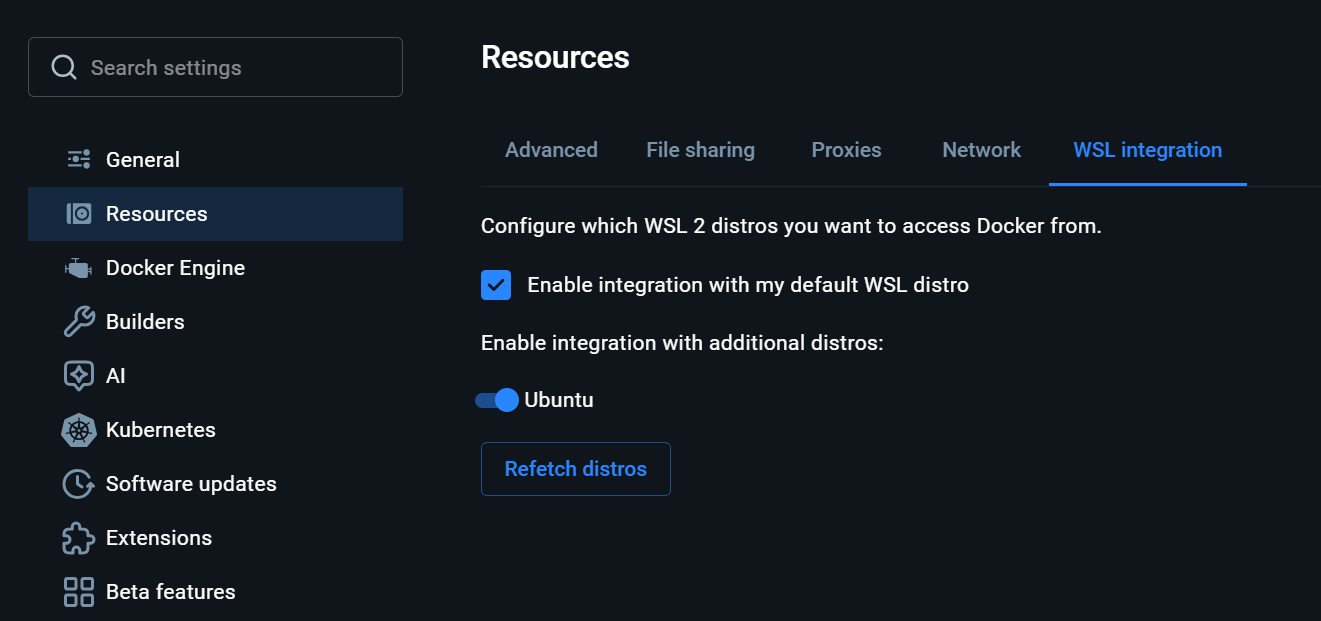
\includegraphics[width=0.78\textwidth]{docker_wsl_integration.png}
\caption{Docker Desktop : activer l'intégration WSL pour la distribution Ubuntu.}
\label{fig:wsl}
\end{figure}

\needspace{6\baselineskip}
\textbf{Vérification :} ouvrez un terminal (sous Windows, \cmd{wsl -d Ubuntu}), puis tapez :
\begin{lstlisting}[style=shell]
docker --version
docker compose version
docker run --rm hello-world
\end{lstlisting}

\begin{resultat}
Les deux versions s'affichent, puis le message \texttt{Hello from Docker!} (figure~\ref{fig:verif}).
\end{resultat}

\begin{figure}[H]
\centering
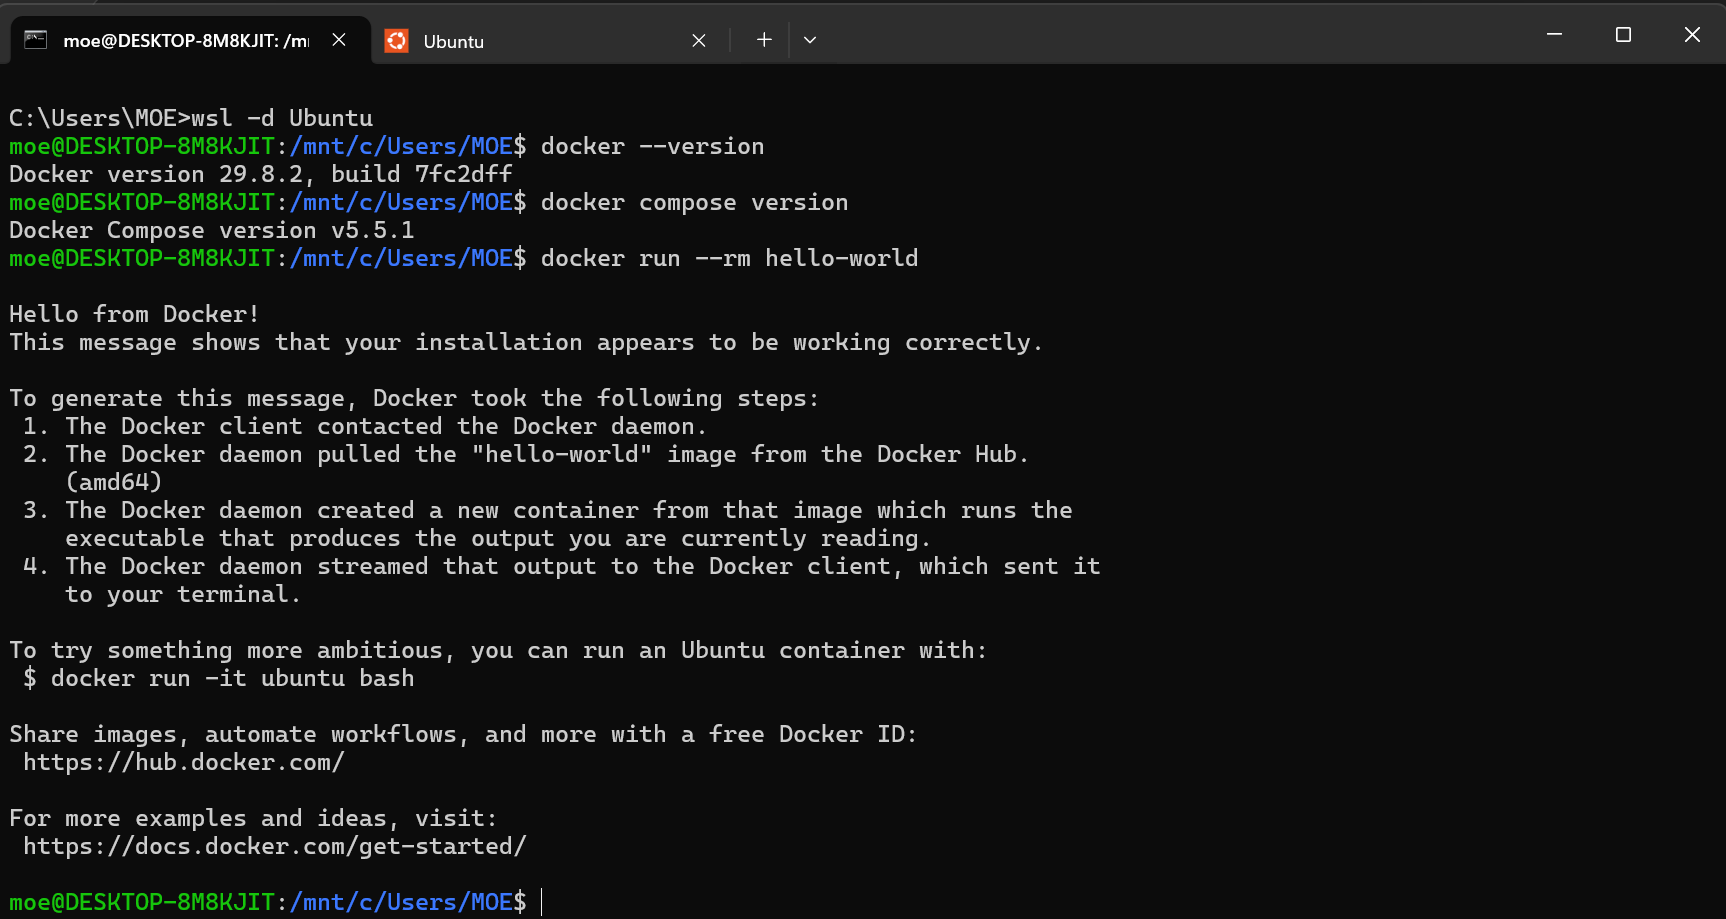
\includegraphics[width=0.85\textwidth]{docker_verification.png}
\caption{Vérification de l'installation de Docker depuis le terminal Ubuntu (WSL).}
\label{fig:verif}
\end{figure}

% =====================================================================
\section{Installer l'environnement du cours}
% =====================================================================

Toutes les commandes s'exécutent dans un terminal (sous Windows, le terminal \textbf{Ubuntu} installé avec WSL).

\subsection*{Étape 1 -- Récupérer le dossier du cours}
\begin{lstlisting}[style=shell]
git clone https://github.com/moeJEE/lakehouse-tp.git
cd lakehouse-tp
\end{lstlisting}
Sans Git : téléchargez le fichier ZIP depuis la page du dépôt et décompressez-le.
Le contenu du dossier est décrit à la section~\ref{sec:depot}.

\begin{attention}
Le dépôt est en \textbf{lecture seule} pour vous : vous récupérez le code, vous ne poussez rien
(pas de \cmd{git commit} ni de \cmd{git push}). Votre travail se fait dans le dossier
\cmd{notebooks/mon\_travail/}, que Git ignore, et se rend sur l'espace de cours.
\end{attention}

\subsection*{Étape 2 -- Créer le fichier de configuration}
\begin{lstlisting}[style=shell]
cp .env.example .env
\end{lstlisting}
\textbf{Machine de 8 Go uniquement :} ouvrez \cmd{.env} et remplacez \cmd{JUPYTER\_MEM\_LIMIT=4g} par \cmd{3g}.
Au TP 3, ne faites jamais tourner en même temps Trino et Superset d'un côté, Airflow et la
supervision de l'autre (section~\ref{sec:services}).

\subsection*{Étape 3 -- Télécharger les images (le plus long)}
\begin{lstlisting}[style=shell]
docker compose --profile full --profile orchestration --profile observabilite pull
\end{lstlisting}
Si le téléchargement s'interrompt, relancez simplement la même commande.

\subsection*{Étape 4 -- Démarrer}
\begin{lstlisting}[style=shell]
docker compose up -d
\end{lstlisting}

\subsection*{Étape 5 -- Contrôler l'état des services}
\begin{lstlisting}[style=shell]
docker compose ps
\end{lstlisting}

\begin{resultat}
Après environ une minute, \texttt{rustfs}, \texttt{iceberg-rest}, \texttt{postgres} et \texttt{jupyter}
sont à l'état \texttt{running}. Le service \texttt{init-buckets} est à l'état \texttt{exited (0)}.
C'est normal, il a préparé le stockage puis s'est arrêté.
\end{resultat}

\needspace{22\baselineskip}
\subsection*{Étape 6 -- Lancer le test automatique}
\begin{lstlisting}[style=shell]
docker compose exec jupyter python /opt/lakehouse/scripts/check_env.py
\end{lstlisting}

\begin{resultat}
\begin{lstlisting}[basicstyle=\ttfamily\footnotesize,backgroundcolor=\color{white},frame=none]
[OK] 1. Stockage S3 (RustFS)
[OK] 2. Catalogue Iceberg REST
[OK] 3. PostgreSQL
[OK] 4. Spark + Iceberg
[OK] 5. Spark + Delta Lake
[OK] 6. DuckDB lit les fichiers sur S3
[OK] 7. dbt (adaptateurs spark et trino)
[--] 8. Trino (profil sql/full non démarré ?)
[--] 9. Airflow (profil orchestration non démarré ?)
[--] 10. Prometheus (profil observabilite non démarré ?)
[--] 11. Mesure des conteneurs (profil observabilite non démarré ?)
[--] 12. Grafana (profil observabilite non démarré ?)
[--] 13. Marquez (lineage) (profil observabilite non démarré ?)
ENVIRONNEMENT PRÊT
\end{lstlisting}
\textbf{Faites une capture d'écran de ce résultat}, elle figurera dans votre compte rendu.
La ligne 8 en \texttt{[--]} est normale : pour économiser la mémoire, Trino et Superset
\textbf{ne démarrent pas automatiquement}. Vous en aurez besoin au TP 3. Vérifiez donc dès
maintenant qu'ils fonctionnent, en les lançant puis en refaisant le test :
\begin{lstlisting}[style=shell]
docker compose --profile full up -d
\end{lstlisting}
La ligne 8 passe alors en \texttt{[OK]}. Arrêtez-les ensuite avec
\cmd{docker compose -{}-profile full stop trino superset}.
\end{resultat}

\subsection*{Étape 7 -- Vérifier les outils du TP 3 (conseillé)}
Les lignes 9 à 13 concernent les outils du TP 3. Vérifiez une fois qu'ils démarrent sur votre
machine, puis arrêtez-les :
\begin{lstlisting}[style=shell]
docker compose --profile orchestration --profile observabilite up -d
docker compose exec jupyter python /opt/lakehouse/scripts/check_env.py
docker compose --profile orchestration --profile observabilite stop
\end{lstlisting}

\begin{resultat}
Attendez une à deux minutes avant le test, le temps qu'Airflow et Marquez préparent leur base au
premier démarrage. Les lignes 9 à 13 passent alors en \texttt{[OK]}, et seule la ligne 8 reste en
\texttt{[--]}.
\end{resultat}

% =====================================================================
\section{Le contenu du dépôt}\label{sec:depot}
% =====================================================================

Le dossier \cmd{lakehouse-tp} récupéré à l'étape~1 est organisé comme suit. Les noms en gras
sont des dossiers, et les fichiers sont décalés sous le dossier qui les contient.

\newcommand{\dossier}[2][0]{\hspace*{#1em}\textbf{\texttt{#2}}}
\newcommand{\fic}[2][1.2]{\hspace*{#1em}\texttt{#2}}

{\small
\renewcommand{\arraystretch}{1.2}
\begin{xltabular}{\textwidth}{@{}>{\raggedright\arraybackslash}p{5.6cm} >{\raggedright\arraybackslash}X@{}}
\toprule
\textbf{Élément} & \textbf{Rôle} \\
\midrule
\endfirsthead
\toprule
\textbf{Élément} & \textbf{Rôle} \\
\midrule
\endhead
\bottomrule
\endfoot
\dossier{lakehouse-tp/} & Racine du dépôt. \\
\fic{README.md} & Page d'accueil du dépôt sur GitHub, avec le démarrage rapide et les règles. \\
\fic{docker-compose.yml} & Description de tous les services (stockage, catalogue, PostgreSQL,
  JupyterLab, Trino, Superset, Airflow, supervision, Marquez), avec leurs images, ports, volumes et profils. \\
\fic{.env.example} & Modèle de configuration (versions des images, identifiants locaux, ports,
  limites de mémoire), copié en \cmd{.env} à l'étape~2. \\
\fic{.gitignore} & Liste des fichiers que Git ignore, dont \cmd{.env} et \cmd{notebooks/mon\_travail/}. \\
\fic{.gitattributes} & Empêche Git de modifier les fins de ligne des fichiers CSV. \\
\addlinespace
\dossier[1.2]{.github/workflows/} & \\*
\fic[2.4]{*.yml} & Automatisations GitHub Actions (construction des images JupyterLab, Superset et
  Airflow, préparation des données), réservées à l'enseignant. \\
\addlinespace
\dossier[1.2]{docker/} & Recettes de construction des images du cours. \\*
\fic[2.4]{jupyter/Dockerfile} & Image JupyterLab, avec Java, Spark, les connecteurs Iceberg, Delta Lake
  et S3, les bibliothèques Python et dbt. \\
\fic[2.4]{jupyter/requirements.txt} & Liste des bibliothèques Python et de leurs versions. \\
\fic[2.4]{superset/Dockerfile} & Image Superset avec le pilote Trino. \\
\fic[2.4]{superset/superset-init.sh} & Initialisation de Superset au premier démarrage
  (base interne, compte \texttt{admin}). \\
\fic[2.4]{airflow/} & Image Airflow, construite sur l'image JupyterLab (TP 3). \\
\addlinespace
\dossier[1.2]{conf/} & Fichiers de configuration lus par les services au démarrage. \\*
\fic[2.4]{spark/} & Réglages de Spark dans JupyterLab. \texttt{spark-defaults.conf} configure le
  catalogue \texttt{lakehouse}, l'accès au stockage S3 et les extensions Iceberg et Delta, et
  \texttt{log4j2.properties} règle le niveau des messages affichés. \\
\fic[2.4]{trino/catalog/} & Catalogues SQL visibles dans Trino : \\*
\fic[3.6]{lakehouse.properties} & connexion au même catalogue Iceberg que Spark ; \\
\fic[3.6]{postgres.properties} & la base PostgreSQL du TP 1 (fédération, TP 3) ; \\
\fic[3.6]{tpch.properties} & jeu de données de démonstration intégré à Trino. \\
\fic[2.4]{spark-airflow/} & Réglages de Spark pour les tâches Airflow, avec l'envoi du lineage (TP 3). \\
\fic[2.4]{prometheus/} & Sources de métriques collectées (\texttt{prometheus.yml}) et traduction des
  métriques d'Airflow (\texttt{statsd\_mapping.yml}), pour le TP 3. \\
\fic[2.4]{grafana/} & Tableau de bord \og Lakehouse -- supervision \fg{}, source de données et
  alerte \og Exécution de DAG en échec \fg{}, chargés au démarrage de Grafana (TP 3). \\
\fic[2.4]{marquez/marquez.yml} & Configuration de Marquez, dont la base est rangée dans le PostgreSQL du cours (TP 3). \\
\fic[2.4]{dbt/profiles.yml} & Connexions de dbt, avec une cible \texttt{spark} et une cible \texttt{trino} (TP 2 et 3). \\
\addlinespace
\dossier[1.2]{scripts/} & Scripts Python exécutés dans le conteneur JupyterLab. \\*
\fic[2.4]{init\_buckets.py} & Crée les espaces de stockage \texttt{landing} et \texttt{lakehouse}
  (lancé automatiquement par le service \texttt{init-buckets}). \\
\fic[2.4]{check\_env.py} & Test automatique de l'environnement (étape~6). \\
\fic[2.4]{load\_postgres.py} & Charge les données Olist dans PostgreSQL, en deux lots (TP 1). \\
\fic[2.4]{deposer\_photos.py} & Dépose un lot de photos dans la zone d'atterrissage (TP 3). \\
\fic[2.4]{mesurer\_conteneurs.py} & Service de mesure de la mémoire et du processeur des conteneurs,
  pour Prometheus (TP 3). \\
\fic[2.4]{init\_bases.py} & Crée dans PostgreSQL la base de Marquez (TP 3, automatique). \\
\fic[2.4]{generer\_suivi.py}, \dots & Scripts de préparation des données, réservés à l'enseignant. \\
\addlinespace
\dossier[1.2]{data/olist/} & Jeu de données Olist (commerce en ligne brésilien). \\*
\fic[2.4]{*.csv} & Les fichiers de données (commandes, clients, produits, paiements, avis en
  portugais et traduits en anglais, etc.). \\
\fic[2.4]{suivi/} & Messages JSON du suivi des colis (TP 2). \\
\fic[2.4]{README.md} & Provenance et licence des données (CC BY-NC-SA 4.0). \\
\addlinespace
\dossier[1.2]{data/catalogue/} & Photos et fiches produits (TP 3), issues d'Amazon Berkeley Objects. \\
\dossier[1.2]{data/modeles/} & Modèle de vision MobileNet, au format ONNX (TP 3). \\
\addlinespace
\dossier[1.2]{notebooks/} & \\*
\fic[2.4]{tp1/}, \texttt{tp2/}, \texttt{tp3/} & Énoncés des TP (notebooks, projet dbt du TP 2, scripts
  du pipeline et DAG du TP 3), à copier sans les modifier. \\
\fic[2.4]{\textbf{mon\_travail/}} & \textbf{Votre dossier de travail}, ignoré par Git. Vous y copiez
  les énoncés et y écrivez votre code. \\
\addlinespace
\dossier[1.2]{apps/} & \\*
\fic[2.4]{dashboard\_tp1.py}, \dots & Squelettes des tableaux de bord Streamlit des TP 1 et 2, à copier sans les modifier. \\
\addlinespace
\dossier[1.2]{docs/} & Supports du module (sources \LaTeX{}) et leurs images. \\*
\end{xltabular}
}

\textbf{À retenir :} vous ne modifiez que deux choses, le fichier \cmd{.env} (créé à l'étape~2)
et le contenu de \cmd{notebooks/mon\_travail/}. Tout le reste appartient au cours et se met à jour
avec \cmd{git pull}. Les fichiers vides \cmd{.gitkeep} servent seulement à faire exister un dossier
vide dans Git.

% =====================================================================
\section{Ouvrir les outils}
% =====================================================================

\begin{center}
\renewcommand{\arraystretch}{1.25}
\begin{tabularx}{\textwidth}{@{}l l X@{}}
\toprule
\textbf{Outil} & \textbf{Adresse dans le navigateur} & \textbf{Connexion} \\
\midrule
JupyterLab        & \url{http://localhost:8888} & jeton : \texttt{lakehouse} \\
Stockage S3       & \url{http://localhost:9001} & \texttt{lakehouse} / \texttt{lakehouse-secret} \\
Spark UI          & \url{http://localhost:4040} & visible pendant qu'un notebook Spark tourne \\
Trino$^{1}$       & \url{http://localhost:8080} & nom d'utilisateur libre \\
Superset$^{1}$     & \url{http://localhost:8088} & \texttt{admin} / \texttt{admin} \\
Airflow$^{2}$    & \url{http://localhost:8085} & sans mot de passe \\
Prometheus$^{3}$ & \url{http://localhost:9090} & sans mot de passe \\
Grafana$^{3}$ & \url{http://localhost:3000} & \texttt{admin} / \texttt{admin} \\
Marquez$^{3}$ & \url{http://localhost:3001} & sans mot de passe \\
\bottomrule
\end{tabularx}

\smallskip
{\footnotesize $^{1}$ Après \cmd{docker compose -{}-profile full up -d}. \quad
$^{2}$ Après \cmd{docker compose -{}-profile orchestration up -d} (TP 3). \quad
$^{3}$ Après \cmd{docker compose -{}-profile observabilite up -d} (TP 3).}
\end{center}

% =====================================================================
\section{Premier test dans JupyterLab}
% =====================================================================

Dans JupyterLab, créez un notebook dans le dossier \texttt{notebooks/mon\_travail/} et exécutez ces trois cellules.

\textbf{Cellule 1 -- Démarrer Spark}
\begin{lstlisting}[language=Python]
from pyspark.sql import SparkSession
spark = SparkSession.builder.appName("premier_test").getOrCreate()
\end{lstlisting}

\needspace{10\baselineskip}
\textbf{Cellule 2 -- Créer une table, puis la modifier}
\begin{lstlisting}[language=Python]
spark.sql("CREATE NAMESPACE IF NOT EXISTS lakehouse.bronze")

spark.sql("""
    CREATE OR REPLACE TABLE lakehouse.bronze.villes
    (nom STRING, population BIGINT) USING iceberg
""")

spark.sql("""
    INSERT INTO lakehouse.bronze.villes
    VALUES ('Paris', 2100000), ('Lyon', 520000)
""")

spark.sql("""
    UPDATE lakehouse.bronze.villes
    SET population = 2133000
    WHERE nom = 'Paris'
""")

spark.table("lakehouse.bronze.villes").show()
\end{lstlisting}

\textbf{Cellule 3 -- Voir l'historique de la table}
\begin{lstlisting}[language=Python]
spark.sql("""
    SELECT committed_at, operation
    FROM lakehouse.bronze.villes.snapshots
""").show()
\end{lstlisting}

\begin{resultat}
La cellule 3 affiche \textbf{deux versions} de la table : l'insertion, puis la modification.
Un Lakehouse garde l'historique des données, et vous l'exploiterez dans le TP 1.
\end{resultat}

% =====================================================================
\section{Quels services pour quelle partie}\label{sec:services}
% =====================================================================

Chaque outil consomme de la mémoire, donc on ne démarre que ceux dont la partie a besoin. Les
supports des TP rappellent ces commandes au bon moment.

\begin{center}
\small
\renewcommand{\arraystretch}{1.25}
\begin{tabularx}{\textwidth}{@{}l X l l@{}}
\toprule
\textbf{Partie} & \textbf{Services utilisés} & \textbf{Profils à démarrer} & \textbf{Profils à arrêter} \\
\midrule
TP 1, TP 2               & base                                        & --                                  & -- \\
TP 3, partie 1           & base                                        & --                                  & -- \\
TP 3, parties 2 et 3     & base + Airflow                              & \cmd{orchestration}                 & -- \\
TP 3, partie 4           & base + Trino + Superset                     & \cmd{full}                          & \cmd{orchestration} \\
TP 3, partie 5           & base + Airflow + supervision et Marquez     & \cmd{observabilite}, \cmd{orchestration} & \cmd{full} \\
\bottomrule
\end{tabularx}
\end{center}

Pour démarrer ou arrêter un profil :
\begin{lstlisting}[style=shell]
docker compose --profile orchestration up -d      # démarrer (ici Airflow)
docker compose --profile full stop                # arrêter (ici Trino et Superset)
\end{lstlisting}
En partie 5, redémarrez Airflow \emph{après} avoir lancé la supervision
(\cmd{docker compose -{}-profile orchestration restart airflow}), car il ne cherche le service de
métriques qu'à son démarrage.

% =====================================================================
\section{Commandes utiles au quotidien}
% =====================================================================

\begin{center}
\renewcommand{\arraystretch}{1.25}
\begin{tabularx}{\textwidth}{@{}l >{\ttfamily}X@{}}
\toprule
\textbf{Je veux\dots} & \textbf{\normalfont Commande} \\
\midrule
Démarrer                           & docker compose up -d \\
Démarrer avec Trino et Superset    & docker compose -{}-profile full up -d \\
Démarrer Airflow (TP 3)            & docker compose -{}-profile orchestration up -d \\
Démarrer la supervision (TP 3)     & docker compose -{}-profile observabilite up -d \\
Arrêter un groupe d'outils         & docker compose -{}-profile observabilite stop \\
Voir l'état des services           & docker compose -{}-profile full -{}-profile orchestration -{}-profile observabilite ps -a \\
Voir les erreurs d'un service      & docker compose logs -{}-tail 50 jupyter \\
Récupérer les mises à jour du cours & git pull \quad \textrm{puis} \quad docker compose up -d \\
Arrêter (en gardant mes données)   & docker compose -{}-profile full -{}-profile orchestration -{}-profile observabilite down \\
\bottomrule
\end{tabularx}
\end{center}

\begin{attention}
N'ajoutez \textbf{jamais} l'option \cmd{-v} à \cmd{docker compose down}, car elle efface toutes les
données du Lakehouse. Vos notebooks, eux, restent dans le dossier \texttt{notebooks/mon\_travail/}.
\end{attention}

% =====================================================================
\section{En cas de problème}
% =====================================================================

\begin{center}
\small
\renewcommand{\arraystretch}{1.3}
\begin{tabularx}{\textwidth}{@{}>{\raggedright\arraybackslash}p{5.2cm} X@{}}
\toprule
\textbf{Ce que vous voyez} & \textbf{Ce qu'il faut faire} \\
\midrule
Un service est à l'état \texttt{Restarting} ou \texttt{Exited} &
  Lire ses messages avec \cmd{docker compose logs -{}-tail 50 <service>}. La cause est presque
  toujours dans les dernières lignes. \\
\texttt{Exited (137)} &
  Le service a manqué de mémoire. Arrêtez les outils dont la partie n'a pas besoin
  (section~\ref{sec:services}), puis relancez-le. \\
\texttt{port is already allocated} &
  Un autre logiciel utilise ce port. Changez la ligne \cmd{PORT\_...} correspondante dans
  \cmd{.env}, puis lancez \cmd{docker compose up -d}. \\
\texttt{Failed to resolve 'trino'} (ou un autre nom de service) dans un notebook &
  Ce service n'est pas démarré. Lancez son profil (section~\ref{sec:services}). \\
Grafana n'affiche aucune métrique d'Airflow &
  Airflow a démarré avant la supervision. Redémarrez-le avec \cmd{docker compose -{}-profile orchestration restart airflow}. \\
\texttt{git pull} refuse de s'exécuter &
  Un fichier du cours a été modifié par erreur. La commande \cmd{git restore .} le rétablit, sans toucher à
  \cmd{notebooks/mon\_travail/}. \\
Un dossier supprimé par erreur dans JupyterLab &
  JupyterLab le déplace dans la corbeille \cmd{notebooks/.Trash-1000/}. Remettez-le en place
  depuis le terminal Ubuntu avec \cmd{mv}. Un fichier du cours se récupère aussi avec
  \cmd{git restore}. \\
\bottomrule
\end{tabularx}
\end{center}

% =====================================================================
\section{Avant la séance 1}
% =====================================================================

\begin{itemize}[leftmargin=*,label=\cocher,itemsep=2pt]
\item Docker fonctionne (\cmd{hello-world} affiche son message)
\item Le test de l'étape 6 affiche \og ENVIRONNEMENT PRÊT \fg{}
\item Avec le profil \cmd{full}, la ligne 8 du test (Trino) passe en \texttt{[OK]}
\item Conseillé : avec les profils \cmd{orchestration} et \cmd{observabilite}, les lignes 9 à 13 passent en \texttt{[OK]}
\item JupyterLab s'ouvre et le premier test fonctionne
\item Le compte rendu est déposé sur l'espace de cours (section~\ref{sec:cr})
\end{itemize}

% =====================================================================
\section{Compte rendu}\label{sec:cr}
% =====================================================================

Au format PDF, nommé \cmd{NOM\_Prenom\_Support0.pdf}, il contient :
\begin{enumerate}[leftmargin=*,itemsep=2pt]
  \item la capture d'écran du test de l'étape 6 et celle du premier test dans JupyterLab ;
  \item votre configuration (système d'exploitation, mémoire vive, profils lancés) ;
  \item les problèmes rencontrés pendant l'installation et la façon dont vous les avez résolus
        (\og aucun \fg{} est une réponse acceptée) ;
  \item en quelques lignes et avec vos mots, le rôle du stockage S3, du catalogue et de Spark,
        et ce que montre l'historique de la table \cmd{villes}.
\end{enumerate}

\end{document}
